\documentclass[a4paper]{article}

\usepackage[utf8]{inputenc}
\usepackage[portuges]{babel}
\usepackage{a4wide}
\usepackage{multicol}
\usepackage{spverbatim}
\usepackage{graphicx}

\title{Projeto de POO - UMER\\Grupo x}
\author{Sérgio Jorge (A77730) \and Vítor Castro (A77870) \and Marcos Pereira (A79116)}
\date{}


\begin{document}

\maketitle

\begin{abstract}
Neste relatório faremos uma análise do projeto de Programação Orientada aos Objetos, no qual o objetivo era desenvolver um programa, em Java, que fizesse a gestão da \textit{UMER},  uma empresa de transporte de passageiros. Assim, este documento apresenta detalhadamente a abordagem tomada ao problema proposto pela equipa docente da UC.
\end{abstract}

\tableofcontents

\section{Introdução}
\label{sec:intro}

Este projeto foi realizado com o objetivo de desenvolver um programa responsável por toda a gestão de uma empresa de taxis. Foram, então, propostas pelos professores algumas funcionalidades com contexto real enquadradas no tema, às quais o programa deve responder com sucesso. A implementação destas permitiram consolidar e adquirir conhecimentos ao nível da sintaxe de programação em Java e também incentivaram à exploração de estruturas de dados e de bibliotecas características desta linguagem. 
Assim, de modo a facilitar a compreensão do projeto, o relatório está dividido da seguinte forma:

\begin{description}
    \item[Secção 2 :] Problema;
    \item[Secção 3 :] Solução;
    \item[Secção 4 :] Conclusão.
\end{description}
\pagebreak

\section{Problema}
\label{sec:problema}
Neste projeto de POO pede-se para desenvolver um programa capaz de auxiliar na gestão de uma empresa de transporte de pessoas. Assim, este deve ser capaz de:


\begin{itemize}
\item Registar um utilizador (cliente ou motorista);
\item Implementar login no sistema;
\item Criar viaturas;
\item Associar motoristas a viaturas;
\item Um cliente pode solicitar uma viagem escolhendo uma viatura específica ou a mais próxima de si;
\item Classificar o motorista, após a viagem;
\item Registar um utilizador (cliente ou motorista);
\item Possibilidade do cliente conseguir ver as viagens que já fez;
\item Possibilidade do motorista conseguir ver as viagens que já fez;
\item Indicar o total faturado pela viatura ou pela empresa;
\item Listar os 10 clientes que mais gastam;
\item Listar os 5 motoristas que apresentam mais desvios entre valores previstos para a viagem e o valor final faturado;
\item Gravar o estado do programa em ficheiro.

\end{itemize}

\section{Solução}
A nossa solução foi implementada com base em diferentes classes dos quais destacamos:

\begin{itemize}
    \item User;
         \begin{itemize}
         \item{Driver;}
         \item{Client;}
         \end{itemize}
    \item Vehicle;
    \item Trip;
    \item IO.
\end{itemize}
\label{sec:solucao}

\begin{figure}[htbp]
    \centering
    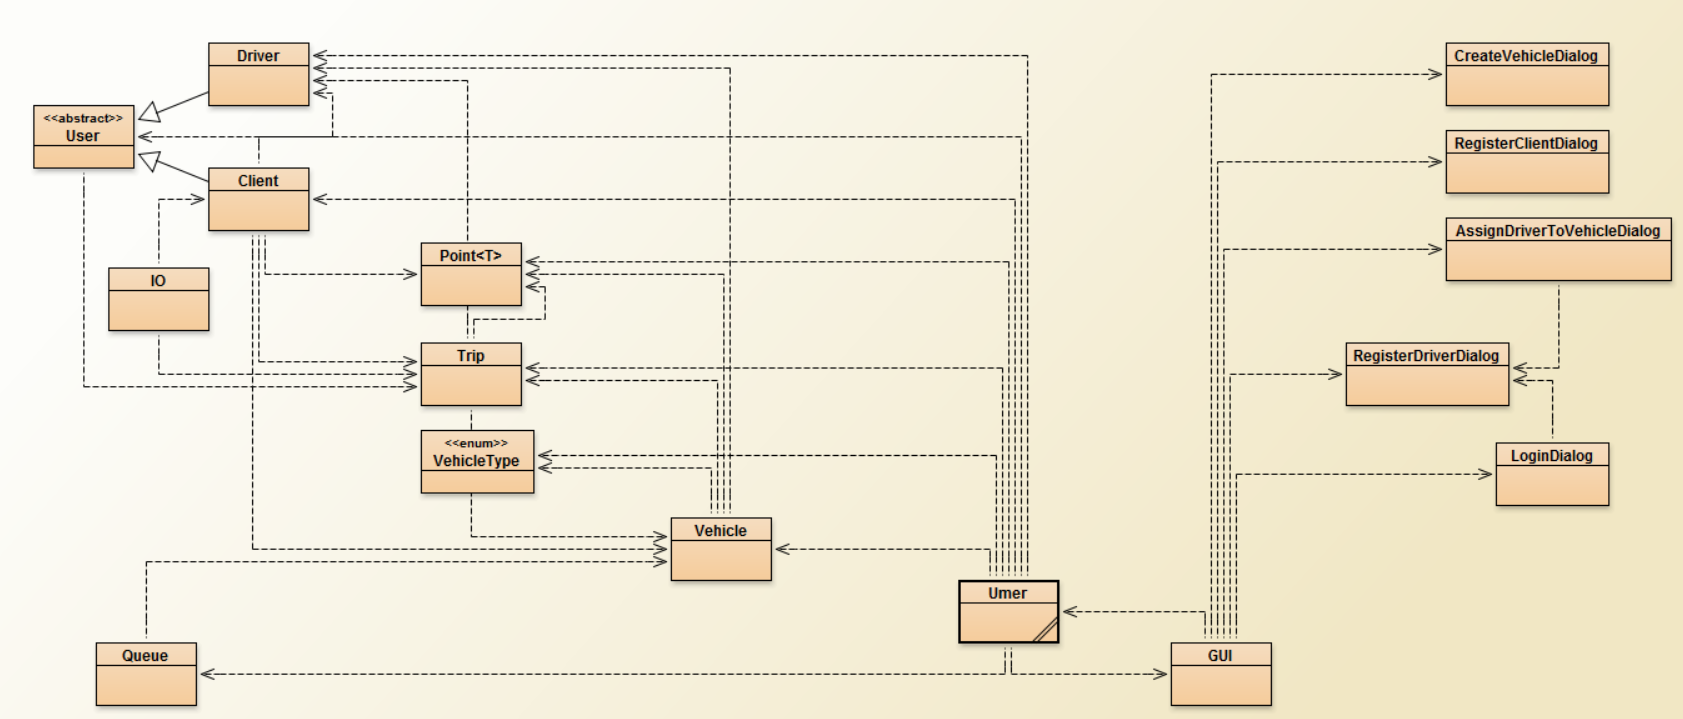
\includegraphics[width = 420pt, height = 240pt]{lala}
\end{figure}

\pagebreak

\subsection{User}
Esta é uma superclasse que define variáveis como: email, nome, password, morada e data de nascimento do utilizador. A razão para a implementação de uma hierarquia é porque todos os campos referidos são comuns a motoristas e a clientes pelo que não há a necessidade de repetir código em diferentes classes. Está definida como abstrata porque não haverá necessidade de instanciar Users.

\begin{description}
    \item[Driver] A classe referente aos motoristas inclui as variáveis definidas na superclasse mas também o grau de cumprimento de horário, a classificação do motorista, o total de quilómetros feitos por este na empresa e um booleano que informa sobre a disponibilidade do motorista.

    \item[Client] Na classe de clientes são também incluídas as variáveis definidas em User. Além disso, define-se o ponto/localização do cliente e o dinheiro total gasto por este. Nesta classe, 

\end{description}

\subsection{Vehicle}
Em Vehicle

\subsection{Trip}
Na classe

\subsection{IO}
Esta classe...

\subsection{Implementação - GUI e classe UMER}
EXPLICAAAR MAIN

\pagebreak
\subsection{Resultado Final}

\section{Conclusões}
\label{sec:conclusao}
Este tra

Este projeto serviu para aprofundarmos o conhecimento da linguagem JAVA, assim como as bibliotecas que lhe estão associadas. Achámos que, com a realização de um trabalho deste tipo permite uma consolidação proveitosa da linguagem, não só em termos teóricos como também em termos práticos. Permite também melhorar as habilidades na resolução de problemas. Concluímos também que:

\begin{itemize}
        \item jhjh
 	    \item jkjskdj
\end{itemize}

\end{document}